%%%%%%%%%%%%%%%%%%%%%%%%%%%%%%%%%%%%%%%%%%%%%%%%%%%%%%%%%%%%%%%
%  BDBI Demo Day -- RESEARCH POSTER  (36in wide x 24in tall)
%  FishCast / Fall 2026
%  Compile with pdfLaTeX (Overleaf). Print at 100% / actual size.
%%%%%%%%%%%%%%%%%%%%%%%%%%%%%%%%%%%%%%%%%%%%%%%%%%%%%%%%%%%%%%%
\documentclass{article}
\usepackage[paperwidth=36in, paperheight=24in, margin=0in]{geometry}
\usepackage[compact]{bdbi}

% ----- Project metadata -----
\newcommand{\projtitle}{FishCast:\\[0.12em]
Predicting Climate Change Effects on Marine Population Distributions}
\newcommand{\projauthors}{Brandon Yu, Ayden Khalil, Alfred Ye}
\newcommand{\projaffil}{BDBI \textbullet{} Demo Day 2026 \quad\textbar\quad Lead: Nash Moore}
\newcommand{\demourl}{https://aye1024.github.io/fish-cast/}

% Layout
\newlength{\pad}    \setlength{\pad}{0.55in}
\newlength{\gap}    \setlength{\gap}{0.45in}
\newlength{\headh}  \setlength{\headh}{4.25in}
\newlength{\colw}   \setlength{\colw}{\dimexpr(36in-2\pad-2\gap)/3\relax}
% Leave a small bottom safety margin so columns cannot spill off the page
\newlength{\colh}   \setlength{\colh}{\dimexpr24in-\headh-\pad-0.75in\relax}

\begin{document}
\noindent
\begin{tikzpicture}[remember picture, overlay]
  \fill[bdbiLight] (current page.south west) rectangle (current page.north east);
  \fill[bdbiPrimary] (current page.north west) rectangle ([yshift=-\headh]current page.north east);
  \fill[bdbiAccent] ([yshift=-\headh]current page.north west) rectangle ([yshift=-\headh-0.15in]current page.north east);
  \node[anchor=west] at ([xshift=\pad, yshift=-\headh/2]current page.north west)
    {\placeholder{3.0in}{3.0in}{Logo}};
  \node[anchor=east] at ([xshift=-\pad, yshift=-\headh/2]current page.north east)
    {
\includegraphics[height=2.85in]{figures/qr-github.png}};
  \node[align=center, text=white, text width=24.5in] at ([yshift=-\headh/2]current page.north) {%
    {\fontsize{40}{44}\selectfont\bfseries \projtitle\par}\vspace{0.28em}
    {\LARGE \projauthors\par}\vspace{0.12em}
    {\Large \projaffil\par}};
\end{tikzpicture}%
%
% ================= COLUMN 1 =================
\begin{tikzpicture}[remember picture, overlay]
\node[anchor=north west, inner sep=0pt] at ([xshift=\pad, yshift=-\headh-0.45in]current page.north west) {%
\begin{minipage}[t][\colh][t]{\colw}
  \begin{block}{Introduction}
    Antarctic krill (\textit{Euphausia superba}) feed whales, penguins, and seals, and
    help move carbon into the deep ocean. Warming and sea-ice loss can push populations
    out of fixed CCAMLR Marine Protected Areas (MPAs) into waters that are easier to fish.
    \begin{itemize}\setlength{\itemsep}{0.15em}
      \item \textbf{Question:} Can we forecast krill density and hotspots under future
            climate better than simple baselines?
      \item \textbf{Hard parts:} patchy hauls (36\% zeros), spatial dependence, and the
            need for climate-only skill on future maps.
      \item \textbf{Our add:} a KRILLBASE--CMIP6 pipeline, spatial models, held-out-year
            benchmarks, and MPA-relative maps.
    \end{itemize}
  \end{block}
  \vspace{0.25em}
  \begin{block}{Objectives}
    \begin{enumerate}\setlength{\itemsep}{0.12em}
      \item Clean KRILLBASE--CMIP6 data and a fair train / val / test split.
      \item Train spatial models and score skill on years the model has not seen.
      \item Map forecasts against CCAMLR MPAs to show spillover risk.
    \end{enumerate}
  \end{block}
  \vspace{0.25em}
  \begin{block}{Data}
        \centering
        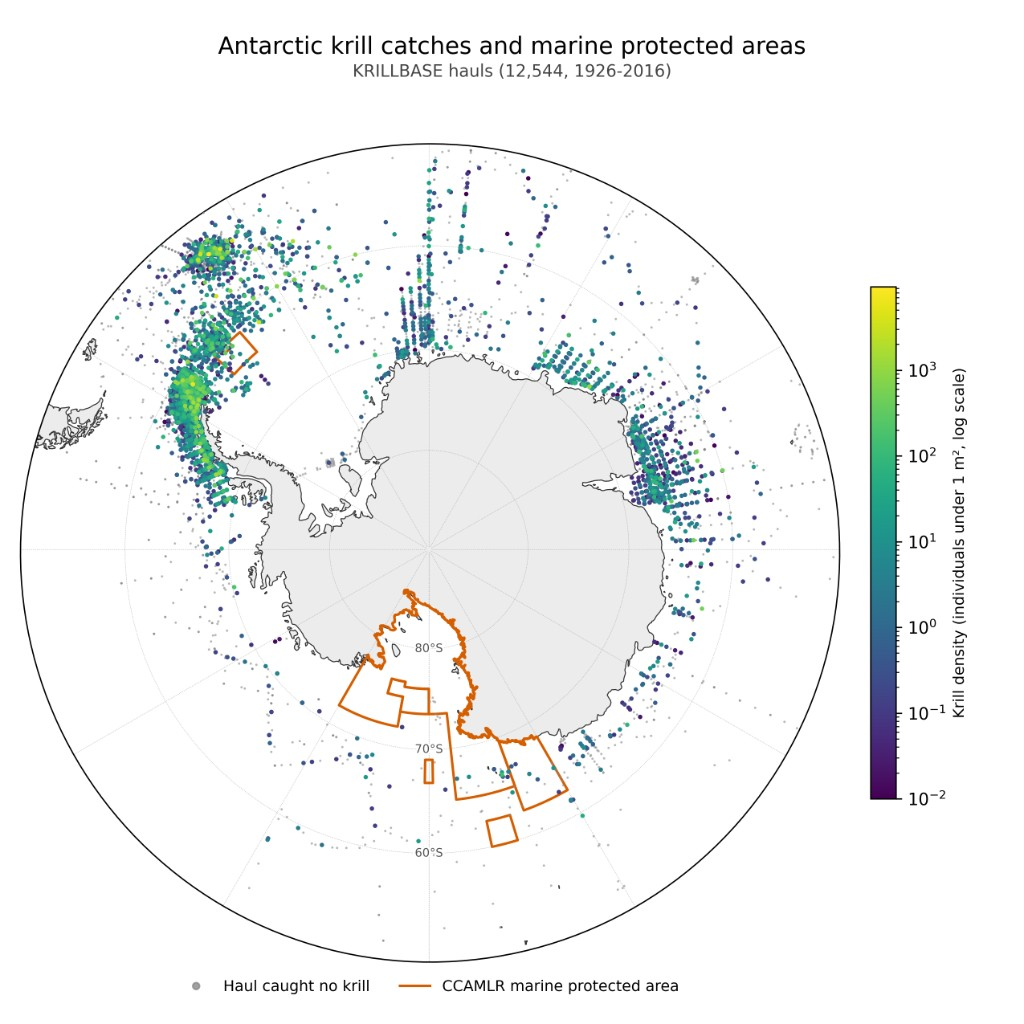
\includegraphics[width=\linewidth]{figures/polar_map.png}\par
        \vspace{0.25em}\raggedright\small
        \textbf{Source:} KRILLBASE + CMIP6 (MPI-ESM1-2-LR).
        \textbf{Size:} 12{,}544 hauls (1926--2016), $\sim$36\% zeros, 7 climate variables.\\
        \textbf{Split:} Train 1926--1998 / val 1998--2004 / test 2004--2016.\\
        \textbf{Fix:} Longitude bug put wrong climate on 77\% of hauls west of Greenwich;
        rebuild uses historical CMIP6 through 2014 and SSP2-4.5 afterward.
  \end{block}
\end{minipage}};
\end{tikzpicture}%
%
% ================= COLUMN 2 =================
\begin{tikzpicture}[remember picture, overlay]
\node[anchor=north, inner sep=0pt] at ([yshift=-\headh-0.45in]current page.north) {%
\begin{minipage}[t][\colh][t]{\colw}
  \begin{block}{Methods}
    \centering
    \resizebox{0.95\linewidth}{!}{\pipeline{11cm}{2.4cm}}\par\vspace{0.35em}
    \raggedright
    \begin{itemize}\setlength{\itemsep}{0.15em}
      \item \textbf{Pre-processing:} Match hauls to climate; polar coords; train-only
            scaling; sea-ice blanks $\to$ 0 when ice area is 0.
      \item \textbf{Models:} Climate-conditioned GP; autoregressive / latent-state GPs;
            sequence and ConvLSTM baselines.
      \item \textbf{Validation:} Year-blocked test (2004--2016). Tracks: \emph{nowcast}
            (lagged krill OK) vs \emph{climate-only} (what a 2040 map can use), vs
            constant and climate-regression baselines.
    \end{itemize}
  \end{block}
  \vspace{0.25em}
  \begin{block}{Results}
    \centering
    % Swap to \includegraphics[width=\linewidth]{figures/main_result.png} when uploaded.
    \placeholder{\linewidth}{5.2in}{Main result figure\\(figures/main\_result.png)}\par
    \vspace{0.25em}\raggedright\small
    Figure 1. Held-out skill: recent-krill models beat a constant; climate-only do not yet.\\[0.2em]
    \textbf{Data validation:} GP test RMSE 1.321 $\to$ 1.285 after preprocessing v2
    (2.7\%). Models with recent catches are $\sim$5\% better than a constant; climate-only
    skill is still near zero.
  \end{block}
  \vspace{0.25em}
  \begin{keybox}
    \centering\large
    Key finding: recent krill history helps nowcasts ($\sim$5\% better than a constant),
    but climate alone does not yet predict held-out years --- so 2040 maps are not ready.
  \end{keybox}
\end{minipage}};
\end{tikzpicture}%
%
% ================= COLUMN 3 =================
\begin{tikzpicture}[remember picture, overlay]
\node[anchor=north east, inner sep=0pt] at ([xshift=-\pad, yshift=-\headh-0.45in]current page.north east) {%
\begin{minipage}[t][\colh][t]{\colw}
  \begin{block}{Demo}
    \centering
    % width-only so the 16:9 screenshot spans the full column
    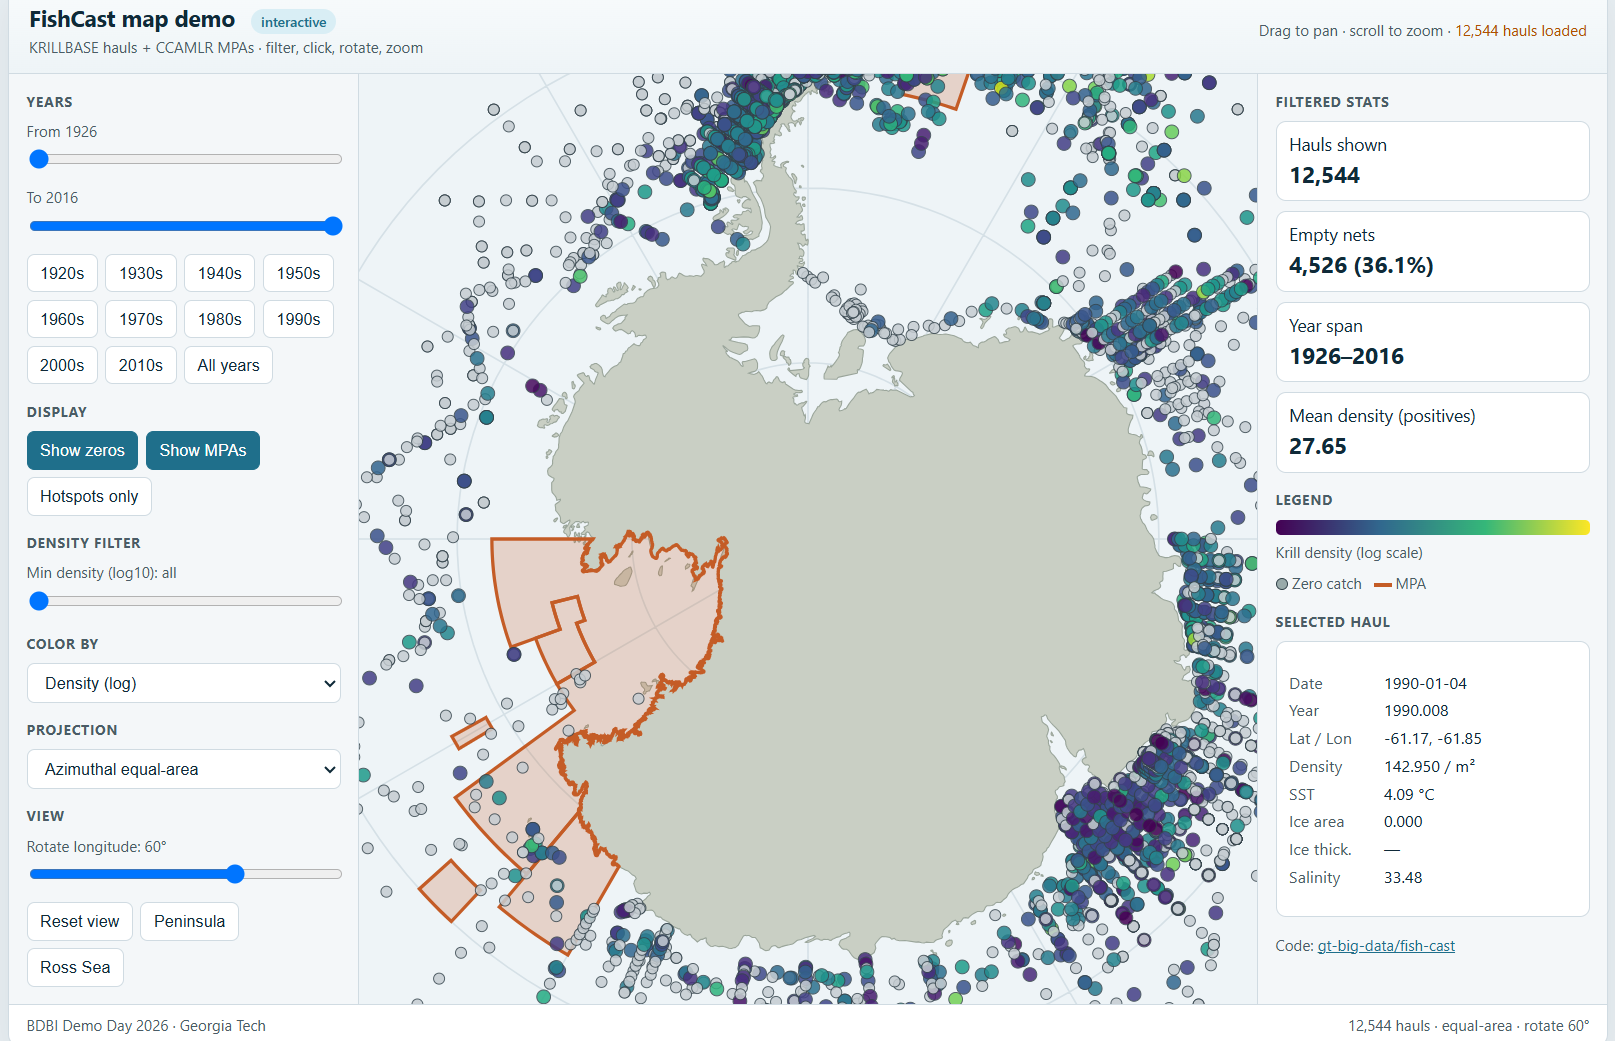
\includegraphics[width=\linewidth]{figures/demo-running.png}\par
    \vspace{0.2em}\raggedright\small
    Figure 2. Interactive map demo: hauls over CCAMLR MPAs. QR (top right) opens the repo.
  \end{block}
  \vspace{0.25em}
  \begin{block}{Conclusions}
    \begin{itemize}\setlength{\itemsep}{0.12em}
      \item Fair pipeline and year split are in place; data bugs hid climate signal.
      \item Autoregressive GPs beat a constant for nowcasts; climate-only models do not.
      \item Without climate skill, warming spillover maps are not yet trustworthy.
    \end{itemize}
  \end{block}
  \vspace{0.25em}
  \begin{block}{Future Work}
    \begin{itemize}\setlength{\itemsep}{0.12em}
      \item Rerun the full benchmark on the longitude-fixed dataset.
      \item Prototype sdmTMB (Tweedie / hurdle) for empty nets.
      \item Use BRT for ice--SST interactions; winter-ice check on future maps.
    \end{itemize}
  \end{block}
  \vspace{0.25em}
  \begin{block}{References \& Acknowledgments}
    \footnotesize
    [1] Atkinson et al.\ KRILLBASE. BAS.\par
    [2] Eyring et al.\ CMIP6 overview. \textit{Geosci.\ Model Dev.} (2016).\par
    [3] Elith et al.\ Boosted regression trees. \textit{J.\ Anim.\ Ecol.} (2008).\par
    [4] Anderson et al.\ sdmTMB spatial GLMMs.\par\vspace{0.25em}
    Thanks to Nash, BDBI, PACE, BAS (KRILLBASE), and Copernicus CDS (CMIP6).
  \end{block}
\end{minipage}};
\end{tikzpicture}%
\end{document}
